\begin{scanpage}{0221}{203}
If in this expansion one limits oneself to the first term, then
\[D(l)=\frac1{3\left(\ln4l-\frac73\right)}.\tag{33.04}\]
The results of numerical calculations based on Equations (33.04) are shown in Figure 75 by the dashed curve: we see that the latter equation gives a good precision already with $l\gtrsim9$.
\begin{center}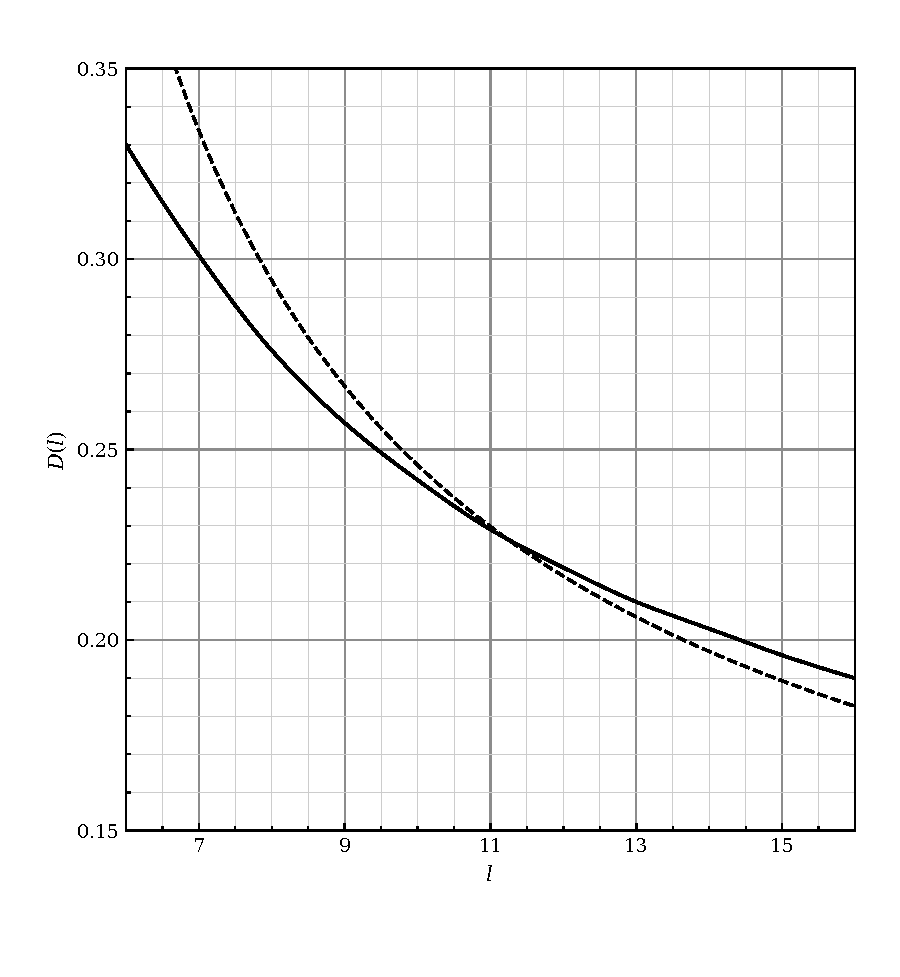
\includegraphics[width=.60\linewidth]{images/recreated/r-0221-fig75.pdf}\par
Figure 75. Graph of the function $D(l)$ which determines the cylinder's dipole moment.\end{center}
Thus, the dipole moment of a vibrator which is short in comparison with the wavelength equals
\[p_z=E\frac{L^3}{24}\frac{\sin\vartheta_0}{\ln\dfrac{2L}a-\dfrac73}\left\{1+O\left[\left(\ln\frac La\right)^{-2}\right]\right\},\tag{33.05}\]
and its scattering characteristic must have the form
\end{scanpage}
